\documentclass[12pt]{article}
% set tiems new roman in latex
\usepackage{newtxtext}
\usepackage[paper=letterpaper,margin=2.54cm]{geometry}
\usepackage{amsmath}
\usepackage{amssymb}
\usepackage{amsfonts}
\usepackage{newtxtext, newtxmath}
\usepackage{enumitem}
\usepackage{titling}
\usepackage[colorlinks=true]{hyperref}
\usepackage{graphicx}
\usepackage{float}
\usepackage{listings}
\usepackage{xcolor}
\usepackage{color}
\usepackage{caption}
\usepackage{subfigure}
\usepackage{float}
\usepackage{booktabs}
\usepackage{multirow}


\setlength{\droptitle}{-6em}
% Enter the specific assignment number and topic of that assignment below, and replace "Your Name" with your actual name.
\title{Project: Comp 6771 Image Processing}
\author{Yunqi Xu 40130514}
\date{\today}


\begin{document}
% \maketitle
\begin{titlepage}
  \rule{\textwidth}{1pt}   % The top horizontal rule
    \vspace{0.2\textheight}  % Whitespace between top horizontal rule and title

    %------------------------------------------------------------
    %    Title
    %------------------------------------------------------------

    {\Huge COMP 6771 Image Processing: Project}

    \vspace{0.025\textheight}   % Whitespace between the title and short horizontal rule

    \rule{0.83\textwidth}{0.4pt}  % The short horizontal rule under title

    \vspace{0.1\textheight}  % Whitespace between the short horizontal rule and author

    %------------------------------------------------------------
    %    Author
    %------------------------------------------------------------

    {\Large Student name: \textsc{Yunqi Xu}}
    \vfill
    {\Large Student id: 40130514}
    \vfill  % Whitespace between author and date

    {\large \today}
    \vspace{0.1\textheight}  % Whitespace between date and bottom horizontal rule

    %------------------------------------------------------------
    %    Bottom rules
    %------------------------------------------------------------

    \rule{\textwidth}{1pt}  % The bottom horizontal rule
\end{titlepage}

\section{Review}
\subsection{Review of Bilateral Filter}
% overall summary of bilateral filter
Bilateral Filter is one of the most important filter method which presented by Tomasi in 1998. 
The bilateral filter smoothing image and preserve edges information at the meanwhile.

% review of the bilateral filter method
The main method that the bilateral filter utilized are two Gaussian filters. 
One is calcualted based on the Geometric closeness. 
Another is calculated based on their photometric similarity
Below is the process of Bilateral Filtering an image:
% add the processing step

% achievement



\subsection{Review of another paper}
% In this section, first introduce another method that provided by other paper, and then compared with the Bilateral filter


\section{Details of Bilateral Filter}
\label{section Bilateral_filter}
% modify with citation of sections
This section contains three main parts. we will firstly present the result of our re-implement method, and then compared the bilater filter with other baseline algorithm in terms of other low pass filters that usually blur the image but also blur edges. 
Finally, we will discuss about the Bilateral filter from both advantages and disadvantages and the difficulties during the implement process.


\subsection{Result of the Re-implement algorithm}
\label{section reimplement}
The main purpose for this section is providing an provement of the successful re-implement of the Bilateral filter.
During our experiment, we use the images from the Bilateral filter paper[cite here], inputted the same parameters that the paper utilized, and compared our result with the oroginal paper and also the build-in function with Opencv-python offcial to prove the successfully re-implement of our code.

\subsubsection{Test result on gray images}
\label{subsection test gray}
Firstly, we present our result compared with the result indicated in the paper, with the same inputted parameters and the same pattern.
In the papre, the author use the parameters $\sigma_d = (1, 3, 10)$ and $\sigma_r = (10, 30, 100, 300)$ correspond to each consisting the parameter set.  
We also use the $kernel\_size = 25$.
The Fig.~\ref{im_cateye} presents the output of our re-implement Bilateral filter.
In this Figure, we can find the blur trend are similar with Figure 3. from the Bilteral filter paper.
The Fig.~\ref{im_cateye_1_10} has the most clean result, but part of small noises still could be find in it. 
On the other hand, the Fig.~\ref{im_cateye_10_300} is the most blur one in these outputs, it only remain a blurry profile of the cat. 

\begin{figure}[H]
  \centering
  \subfigure[$\sigma_d=1, \sigma_r=10$]{
  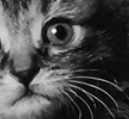
\includegraphics[width=3.5cm]{output_image/cat_part_ds1_rs10.png}
  % \caption{fig1}
  \label{im_cateye_1_10}
  }
  \quad
  \subfigure[$\sigma_d=1, \sigma_r=30$]{
  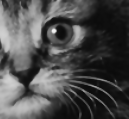
\includegraphics[width=3.5cm]{output_image/cat_part_ds1_rs30.png}
  }
  \quad
  \subfigure[$\sigma_d=1, \sigma_r=100$]{
  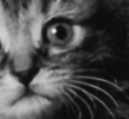
\includegraphics[width=3.5cm]{output_image/cat_part_ds1_rs100.png}
  }
  \quad
  \subfigure[$\sigma_d=1, \sigma_r=300$]{
  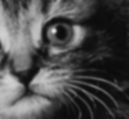
\includegraphics[width=3.5cm]{output_image/cat_part_ds1_rs300.png}
  }

  \subfigure[$\sigma_d=3, \sigma_r=10$]{
  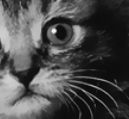
\includegraphics[width=3.5cm]{output_image/cat_part_ds3_rs10.png}
  % \caption{fig1}
  }
  \quad
  \subfigure[$\sigma_d=3, \sigma_r=30$]{
  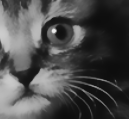
\includegraphics[width=3.5cm]{output_image/cat_part_ds3_rs30.png}
  }
  \quad
  \subfigure[$\sigma_d=3, \sigma_r=100$]{
  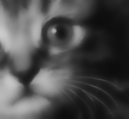
\includegraphics[width=3.5cm]{output_image/cat_part_ds3_rs100.png}
  }
  \quad
  \subfigure[$\sigma_d=3, \sigma_r=300$]{
  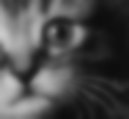
\includegraphics[width=3.5cm]{output_image/cat_part_ds3_rs300.png}
  }

  \subfigure[$\sigma_d=10, \sigma_r=10$]{
  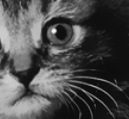
\includegraphics[width=3.5cm]{output_image/cat_part_ds10_rs10.png}
  % \caption{fig1}
  }
  \quad
  \subfigure[$\sigma_d=10, \sigma_r=30$]{
  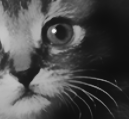
\includegraphics[width=3.5cm]{output_image/cat_part_ds10_rs30.png}
  }
  \quad
  \subfigure[$\sigma_d=10, \sigma_r=100$]{
  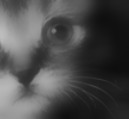
\includegraphics[width=3.5cm]{output_image/cat_part_ds10_rs100.png}
  }
  \quad
  \subfigure[$\sigma_d=10, \sigma_r=300$]{
  
\includegraphics[width=3.5cm]{output_image/cat_part_ds10_rs300.png}
  \label{im_cateye_10_300}
  }
\caption{A detail figure with bilateral filters with various range and domain parameter values by implement code}
\label{im_cateye}
\end{figure}

As the comparison, we also make an experiment of input the same parameter pairs in to the build-in opencv-python funtion to explore whether it will have the same output as our code. Fig.~\ref{py_cateye} prove the results are samilar. 

\begin{figure}[b]
  \centering
  \subfigure[$\sigma_d=1, \sigma_r=10$]{
  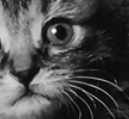
\includegraphics[width=3.5cm]{output_image_python/cat_part_ds1_rs10.png}
  % \caption{fig1}
  }
  \quad
  \subfigure[$\sigma_d=1, \sigma_r=30$]{
  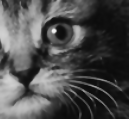
\includegraphics[width=3.5cm]{output_image_python/cat_part_ds1_rs30.png}
  }
  \quad
  \subfigure[$\sigma_d=1, \sigma_r=100$]{
  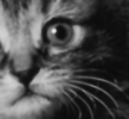
\includegraphics[width=3.5cm]{output_image_python/cat_part_ds1_rs100.png}
  }
  \quad
  \subfigure[$\sigma_d=1, \sigma_r=300$]{
  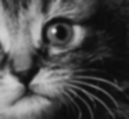
\includegraphics[width=3.5cm]{output_image_python/cat_part_ds1_rs300.png}
  }

  \subfigure[$\sigma_d=3, \sigma_r=10$]{
  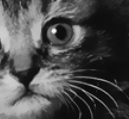
\includegraphics[width=3.5cm]{output_image_python/cat_part_ds3_rs10.png}
  % \caption{fig1}
  }
  \quad
  \subfigure[$\sigma_d=3, \sigma_r=30$]{
  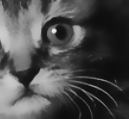
\includegraphics[width=3.5cm]{output_image_python/cat_part_ds3_rs30.png}
  }
  \quad
  \subfigure[$\sigma_d=3, \sigma_r=100$]{
  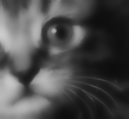
\includegraphics[width=3.5cm]{output_image_python/cat_part_ds3_rs100.png}
  }
  \quad
  \subfigure[$\sigma_d=3, \sigma_r=300$]{
  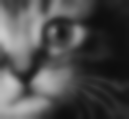
\includegraphics[width=3.5cm]{output_image_python/cat_part_ds3_rs300.png}
  }

  \subfigure[$\sigma_d=10, \sigma_r=10$]{
  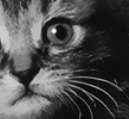
\includegraphics[width=3.5cm]{output_image_python/cat_part_ds10_rs10.png}
  % \caption{fig1}
  }
  \quad
  \subfigure[$\sigma_d=10, \sigma_r=30$]{
  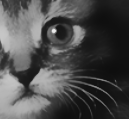
\includegraphics[width=3.5cm]{output_image_python/cat_part_ds10_rs30.png}
  }
  \quad
  \subfigure[$\sigma_d=10, \sigma_r=100$]{
  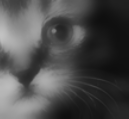
\includegraphics[width=3.5cm]{output_image_python/cat_part_ds10_rs100.png}
  }
  \quad
  \subfigure[$\sigma_d=10, \sigma_r=300$]{
  
\includegraphics[width=3.5cm]{output_image_python/cat_part_ds10_rs300.png}
  }
  \caption{A detail figure with bilateral filters with various range and domain parameter values by Opencv python}
  \label{py_cateye}
  \end{figure}
% Fig.~\ref{py_cateye} indicates that the similarity of output between our re-implement code and the build-in algorithm in python, in other ways prove the successful implement of our code. the output looks very similar.

\begin{figure}[H]
  \centering
  \subfigure[$\sigma_d=1, \sigma_r=10$]{
  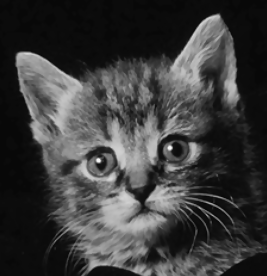
\includegraphics[width=3.5cm]{output_image/cat_ds1_rs10.png}
  % \caption{fig1}
  }
  \quad
  \subfigure[$\sigma_d=1, \sigma_r=30$]{
  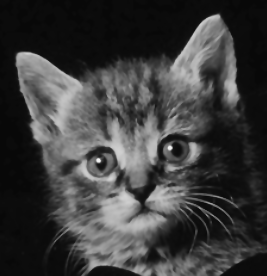
\includegraphics[width=3.5cm]{output_image/cat_ds1_rs30.png}
  }
  \quad
  \subfigure[$\sigma_d=1, \sigma_r=100$]{
  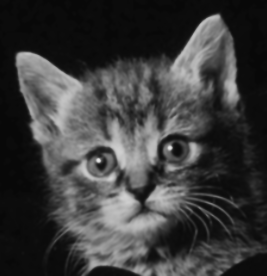
\includegraphics[width=3.5cm]{output_image/cat_ds1_rs100.png}
  }
  \quad
  \subfigure[$\sigma_d=1, \sigma_r=300$]{
  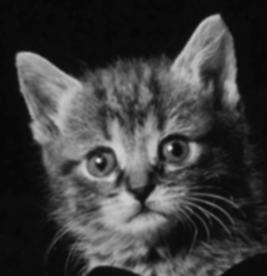
\includegraphics[width=3.5cm]{output_image/cat_ds1_rs300.png}
  }

  \subfigure[$\sigma_d=3, \sigma_r=10$]{
  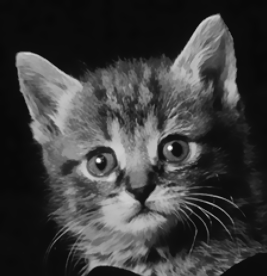
\includegraphics[width=3.5cm]{output_image/cat_ds3_rs10.png}
  % \caption{fig1}
  }
  \quad
  \subfigure[$\sigma_d=3, \sigma_r=30$]{
  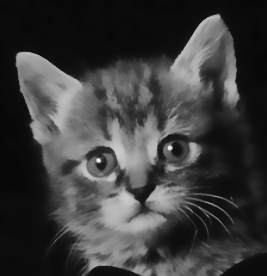
\includegraphics[width=3.5cm]{output_image/cat_ds3_rs30.png}
  }
  \quad
  \subfigure[$\sigma_d=3, \sigma_r=100$]{
  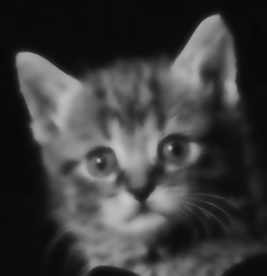
\includegraphics[width=3.5cm]{output_image/cat_ds3_rs100.png}
  }
  \quad
  \subfigure[$\sigma_d=3, \sigma_r=300$]{
  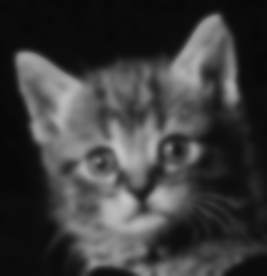
\includegraphics[width=3.5cm]{output_image/cat_ds3_rs300.png}
  }

  \subfigure[$\sigma_d=10, \sigma_r=10$]{
  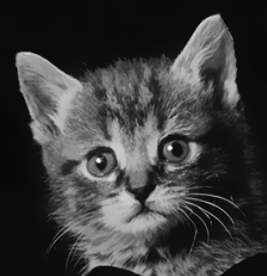
\includegraphics[width=3.5cm]{output_image/cat_ds10_rs10.png}
  % \caption{fig1}
  }
  \quad
  \subfigure[$\sigma_d=10, \sigma_r=30$]{
  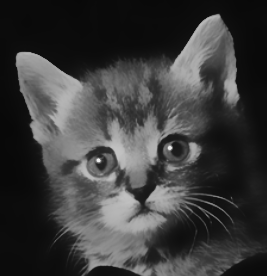
\includegraphics[width=3.5cm]{output_image/cat_ds10_rs30.png}
  }
  \quad
  \subfigure[$\sigma_d=10, \sigma_r=100$]{
  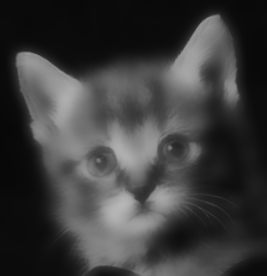
\includegraphics[width=3.5cm]{output_image/cat_ds10_rs100.png}
  }
  \quad
  \subfigure[$\sigma_d=10, \sigma_r=300$]{
  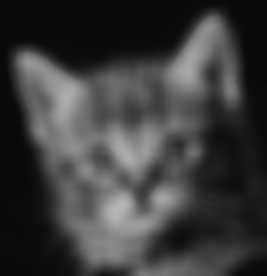
\includegraphics[width=3.5cm]{output_image/cat_ds10_rs300.png}
  }
  \caption{A detail figure with bilateral filters with various range and domain parameter values by re-implement code of cat}
  \label{im_cat}
  \end{figure}

Fig.~\ref{im_cat} are some other outputs use the cat image from paper and the same parameter sets. 
The same as the figures from the paper, some detils, such as the Kitten's whiskers, also can be remained after filtering.

% Fig.~\ref{im_cat} are also two image which prove the success of our re-implement code. 
The Fig.~\ref{snack} are some other outputs use the figures from Bilateral filter paper.  
The Fig.~\ref{snack_original}, ~\ref{snack_onion} are the oroginal images.
As present in Fig.~\ref{snack_original_smooth}, the salt and pepper noise can be removed, at the mean time, the edge information can be keeped as shown in Fig.~\ref{snack_onion_smooth}.
In this experiment, we use same parameters which the paper used. $\sigma_d = 3$ and $\sigma_r = 50$. 


\begin{figure}[H]
  \centering
  \subfigure[Original snack]{
  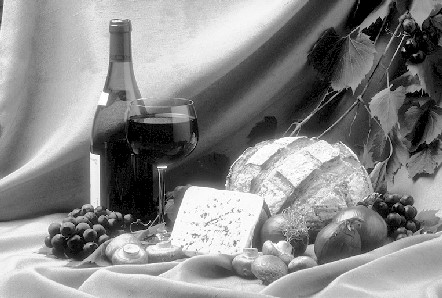
\includegraphics[width=7cm]{original_paper_images/gray/snack.png}
  \label{snack_original}
  }
  \quad
  \subfigure[Smoothed snack]{
  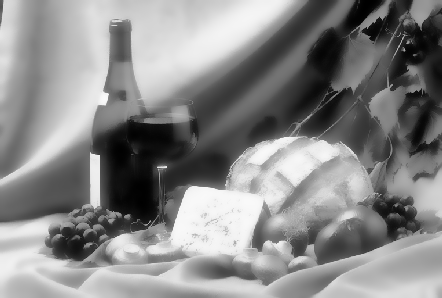
\includegraphics[width=7cm]{output_image/snack_ds3_rs50.png}
  \label{snack_original_smooth}
  }
  \quad
  \subfigure[Original Onion]{
  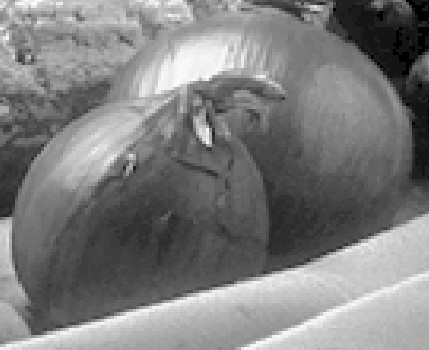
\includegraphics[width=7cm]{original_paper_images/gray/onion.png}
  \label{snack_onion}
  }
  \quad
  \subfigure[Smoothed Onion]{
  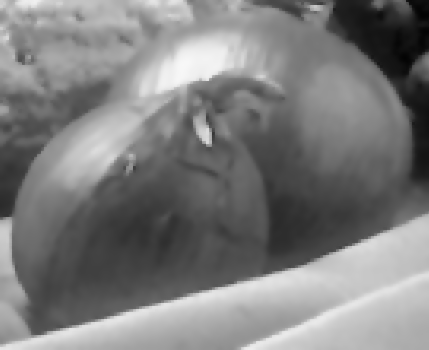
\includegraphics[width=7cm]{output_image/onion_ds3_rs50.png}
  \label{snack_onion_smooth}
  }
  \caption{The Bilater filtering result of snacks and the Onion detail}
  \label{snack}
\end{figure}

\subsubsection{Test result on color images}
The bilateral filter is not only suitable for filtering gray image, but also achieving successful at filtering color images.
Fig.~\ref{color} has presents the result of filtering on color images.
In these images, the left half (Fig.~\ref{color_children}, ~\ref{color_cube}, ~\ref{color_sky}, ~\ref{color_home})are original imput images.
The right half(Fig.~\ref{color_children_smooth}, ~\ref{color_cube_smooth}, ~\ref{color_sky_smooth} and~\ref{color_home_smooth}) are the result of those color images with Bilater filtering. 
Compared with filtering gray images, filtering color images need to convert 3-channels RGB images into the CIE-lab space, and then generate two filters based on geometric and photometric information that an image provided.
Noises on the original input images could be removed.

\begin{figure}[H]
  \centering
  \subfigure[Children]{
  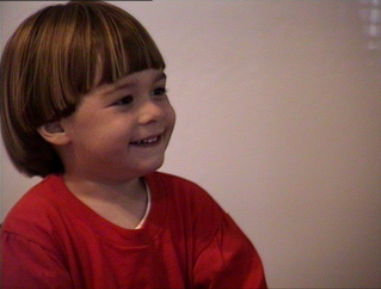
\includegraphics[width=6cm]{original_paper_images/color/child.png}
  \label{color_children}
  }
  \quad
  \subfigure[Smoothed Children]{
  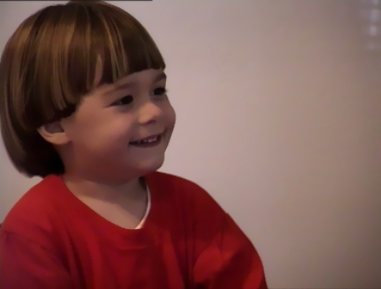
\includegraphics[width=6cm]{output_color_image/child_ds3_rs10.png}
  \label{color_children_smooth}
  }
  \quad
  \subfigure[Rubik's cube]{
  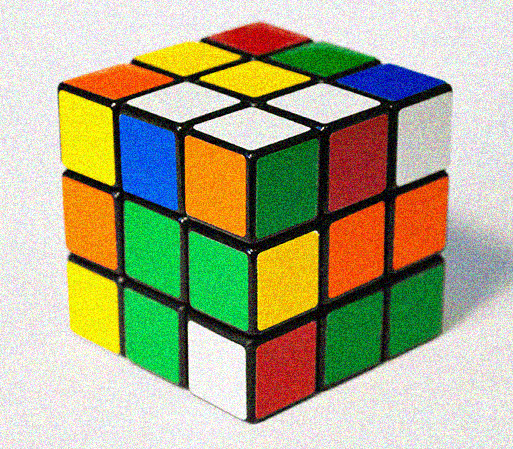
\includegraphics[width=6cm]{original_paper_images/color/rubiks_cube.png}
  \label{color_cube}
  }
  \quad
  \subfigure[Smoothed Rubik's cube]{
  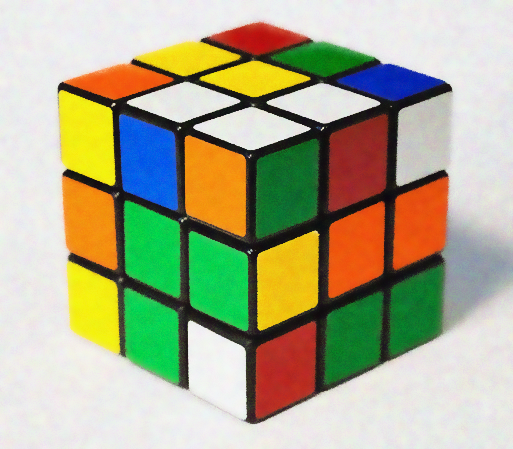
\includegraphics[width=6cm]{output_color_image/rubiks_cube_ds3_rs50.png}
  \label{color_cube_smooth}
  }
  \quad
  \subfigure[Sky]{
  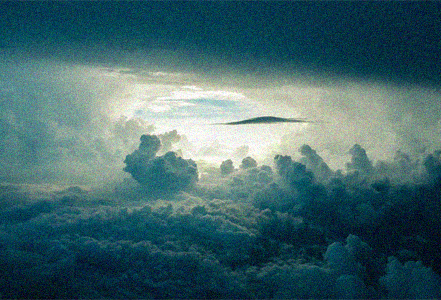
\includegraphics[width=6cm]{original_paper_images/color/sky.png}
  \label{color_sky}
  }
  \quad
  \subfigure[Smoothed sky]{
  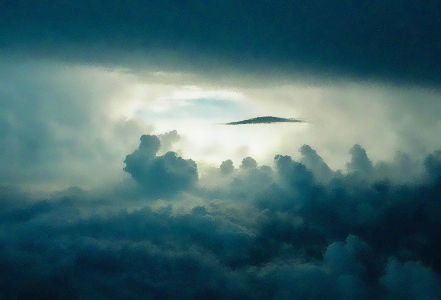
\includegraphics[width=6cm]{output_color_image/sky_ds3_rs30.png}
  \label{color_sky_smooth}
  }
  \quad
  \subfigure[Home]{
  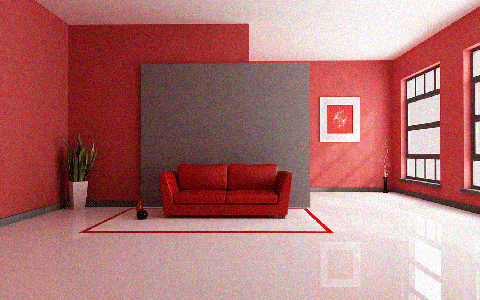
\includegraphics[width=6cm]{original_paper_images/color/home.png}
  \label{color_home}
  }
  \quad
  \subfigure[Smoothed home]{
  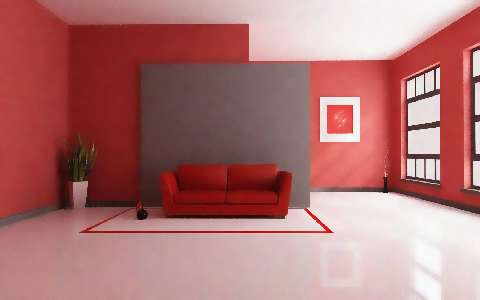
\includegraphics[width=6cm]{output_color_image/home_ds3_rs30.png}
  \label{color_home_smooth}
  }
  \caption{Outputs of color images}
  \label{color}
\end{figure}


\subsection{Compare with other baseline algorithm}
\label{baseline comparison}
% in this section, compared with other blur algorithm
In this section, we compared the filter result of Bilateral filter with other baseline algorithm to present the advantages of our code.
The baseline low-pass filters we used are mean filtering, median filtering and gaussian filtering. 
All of this filters are classic filtering in terms of image processing.
The Section~\ref{section reimplement} not only prove the result of the re-implement code, but also indicate that the general applicability of Bilateral filter.
Our next experiment, we not only compared the output result passed by different filters from human version level, but also calculate the PNSR[cite paper] from mathmatical level. 
The equation of PNSR has been shwo in Eq.~\ref{PSNR equation}:
\begin{equation}
  PSNR = 10\log 10 (\frac{I_{Max}^{2}}{MSE})
  \label{PSNR equation}
\end{equation}

\begin{equation}
  MSE = \frac{\sum_{M, N}[I_1(m,n) - I_2(M, n)]^2}{M * N}
  \label{MSE}
\end{equation}

Where, the $I_{Max}$ is the maximum fluctuation in the input images. 
In our case, the 8-bit integer input image should have $R = 255$.
And the $I_1$ and $I_2$ are the two images between the noisey one and the filtered one.
  
\begin{figure}[H]
  \centering
  \subfigure[mean]{
  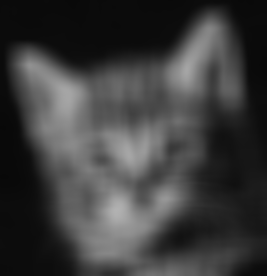
\includegraphics[width=5cm]{output_baseline/cat_mean_25.png}
  \label{gray_baseline_mean}
  }
  \quad
  \subfigure[median]{
  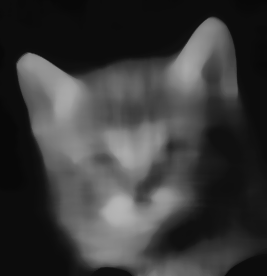
\includegraphics[width=5cm]{output_baseline/cat_median_25.png}
  \label{gray_baseline_median}
  }
  \quad
  \subfigure[gaussian]{
  \includegraphics[width=5cm]{output_baseline/cat_gaussian_25.png}
  \label{gray_baseline_gaussian}
  }
  \quad
  \subfigure[Bilateral filter output]{
  \includegraphics[width=5cm]{output_image/cat_ds10_rs10.png}
  \label{gray_baseline_bilateral}
  }
  \caption{output compared with the baseline low pass filters}
  \label{gray_baseline}
\end{figure}

The Fig.~\ref{gray_baseline} has presented the result between three baseline filters and the Bilateral filter. 
Is is obvious that the the Fig.~\ref{gray_baseline_mean} and Fig.~\ref{gray_baseline_median} get a very bad result, since all the details and texture inforamtions are lose. 
The only remaining parts are the contour in each image.
The result of Gaussian filter, Fig.~\ref{gray_baseline_gaussian} can achieve a very closely result compared with Fig.~\ref{gray_baseline_bilateral}.
However, as we mentioned in Section.~\ref{subsection test gray}, the kitten's whiskers are clean in Fig.~\ref{gray_baseline_bilateral}, they are blured in Fig.~\ref{gray_baseline_gaussian}. 
For further prove our statement, we calculate the PSNR between each output image with filter and the original noisy image.
The Table.~\ref{table_PSNR} presents the PSNR result. 
As the result in the table, the PSNR scores of Median filter and Mean filter are too low to use, but the PSNR score of Gaussian filter can achieve a considerablely compititive result as 31.59, which is higher than using Bilateral filter with $\sigma_s = 3$ and $\sigma_d = 100$ or $\sigma_d = 300$ and $\sigma_s = 10$ and $\sigma_d = 30, 100, 300$. 

\begin{table}[H]
\centering
\begin{tabular}{lllll}
\cline{1-5}
Method & Kernel\_size & sigma\_s & Sigma\_r & PSNR  \\ \cline{1-1}
\cline{1-5}
\multirow{4}{*}{Bilateral Filter}   & \multirow{4}{*}{25} & \multirow{4}{*}    {1}                               & 10      & 42.74 \\
       &             &            & 30      & 32.26     \\
       &             &            & 100     & 32.59     \\
       &             &            & 300     & 31.70     \\
\cline{1-5}
\multirow{4}{*}{Bilateral Filter}   & \multirow{4}{*}{25} & \multirow{4}{*}{3}  & 10       &40.05     \\
      &              &            & 30       & 31.37     \\
      &              &            & 100      & 25.90     \\
      &              &            & 300      & 24.39     \\
\cline{1-5}                                 
\multirow{4}{*}{Bilateral Filteral} & \multirow{4}{*}{25} & \multirow{4}{*}{10} & 10       & 39.62     \\
     &               &            & 30       & 29.72     \\
     &               &            & 100      & 22.38     \\
     &               &            & 300      & 20.31     \\
\cline{1-5}
Median filter       & 25          & None    & None     & 20.31     \\
Mean filter         & 25          & None    & None     & 19.59     \\
Gaussian filter          & 25           & None    & None     & 31.59    
\end{tabular}
\caption{The PSNR output of bailteral filter and baseline filters}
\label{table_PSNR}
\end{table}
The Tabel.~\ref{table_PSNR} presents the PSNR reult compared with Bilater filter and other baseline filters.

% In the experiment, we use $kernel\_size = 25$ for all filters, but the same parameters as before in the paper. 
% The result shows that the bilateral filter has advantages compared with other baseline low-pass filter. 
% Only the Gaussian filter obtains $PSNR = 31.59$ which is very close with some result of the bilater filter and over some bery blur bilateral filters.
% But still not good as the result with some very clean Bilater filters.
%

%------------compare with this baseline filter



\section{Conclusion}
\label{section conclusion}
In this section, we will provide the pros and cons of the methods.
The methods we used in this report that comes from the lecture.
finally, we will provide some brief discription about the difficulties we faced.

\subsection{Pros and Cons}
Pros:

The Bilateral filter can keep the edge meanwhile blur the noise.  

Cons:

When Bilateral neighborhood size gets larger, the Bilateral filtering is slow. 
\subsection{Method used}


\subsection{difficulties}

The first difficulties is implement the $\sigma_r$ in the color image. 
The second is the transform of CIE-lab space. 

\end{document}
